\documentclass[11pt,letterpaper]{article}
\usepackage[margin=.65in,top=.78in,bottom=.65in]{geometry}
\usepackage[T1]{fontenc}
\usepackage{lmodern,tikz,array,fancyhdr}
\usetikzlibrary{arrows.meta}
\renewcommand{\familydefault}{\sfdefault}
\pagestyle{fancy}\fancyhf{}
\fancyhead[L]{\small Week 74 / Doubling elevators / Grades 4--5}
\fancyfoot[L]{\small Bellingham Math Circle / Week 74 / GGT74-S-draft}
\fancyfoot[R]{\small\thepage}
\renewcommand{\headrulewidth}{0pt}\renewcommand{\footrulewidth}{0pt}
\setlength{\parindent}{0pt}\setlength{\parskip}{8pt}
\newcommand{\problem}[2]{\textbf{Problem #1:} #2\par}
\newcommand{\lineblank}{\par\vspace{.35in}\hrule height .25pt\vspace{.15in}}
\newcommand{\board}{
\begin{center}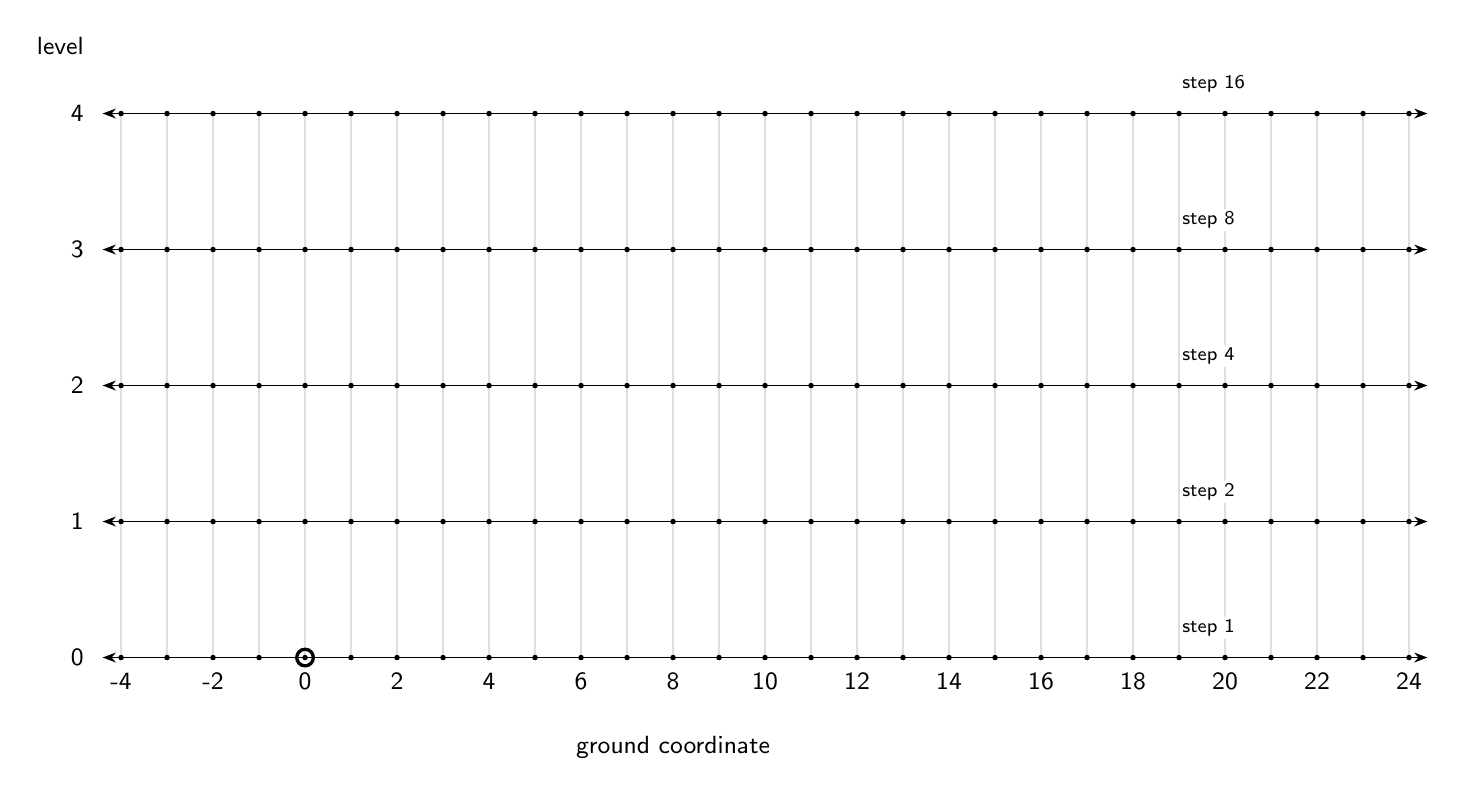
\begin{tikzpicture}[x=.23in,y=.68in,font=\small]
 \foreach \x in {-4,...,24} {\draw[gray!25] (\x,0)--(\x,4);}
 \foreach \h/\step in {0/1,1/2,2/4,3/8,4/16} {
  \draw[<->,>=Stealth] (-4.4,\h)--(24.4,\h);
  \foreach \x in {-4,...,24} {\fill (\x,\h) circle (1pt);}
  \node[anchor=east] at (-4.6,\h) {\h};
  \node[anchor=west,font=\scriptsize,fill=white,inner sep=1pt] at (19,\h+.22) {step \step};
 }
 \foreach \x in {-4,-2,...,24} {\node[below] at (\x,-.04) {\x};}
 \node[anchor=east] at (-4.6,4.5) {level};
 \node at (8,-.66) {ground coordinate};
 \draw[very thick] (0,0) circle (3pt);
\end{tikzpicture}\end{center}}
\begin{document}
Move a pawn. Your partner checks each move and writes its letter.
Swap jobs after a trip. Start at ground coordinate 0, level 0.

U and D move one level straight up or down, keeping the ground coordinate.
Do not go below level 0. R and L move right or left by the level's step size.
Every move costs one. The roads continue beyond this page; higher levels keep doubling.

\begin{center}
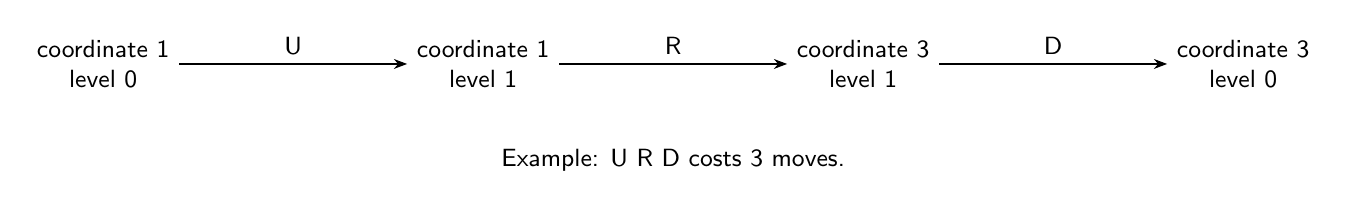
\begin{tikzpicture}[x=.95in,y=.4in,>=Stealth,font=\small]
\node[align=center] (a) at (0,0) {coordinate 1\\level 0};
\node[align=center] (b) at (2,0) {coordinate 1\\level 1};
\node[align=center] (c) at (4,0) {coordinate 3\\level 1};
\node[align=center] (d) at (6,0) {coordinate 3\\level 0};
\draw[->] (a)--node[above]{U}(b);\draw[->](b)--node[above]{R}(c);\draw[->](c)--node[above]{D}(d);
\node at (3,-1.2) {Example: U R D costs 3 moves.};
\end{tikzpicture}
\end{center}
\problem{1}{Reach coordinate 3 and return to level 0 in as few moves as you can. Then try coordinate 7. Your partner may challenge a route with a shorter one.}
\board
3: \hrulefill\par\vspace{.18in}
7: \hrulefill
\newpage
\problem{2}{Reach coordinate 16 and return to level 0. Find the shortest trip you can. Can you find two different trips tied for your best?}
\board
\vspace{.12in}
\begin{tabular}{@{}p{.56\linewidth}p{.32\linewidth}@{}}
Move letters & Number of moves\\[.55in]\hline\\[.4in]\hline\\[.4in]\hline
\end{tabular}\par
\vfill
Shortest trip so far: \rule{1in}{.3pt} moves.
\newpage
\problem{3}{Start at 0 on level 0. With each move budget, finish as far right as possible on level 0. Your partner tries to beat your distance. You may use fewer moves than the budget.}
\vspace{.14in}
\renewcommand{\arraystretch}{1.4}
\begin{tabular}{@{}p{.12\linewidth}p{.54\linewidth}p{.24\linewidth}@{}}
Budget & Move letters & Farthest coordinate\\\hline
4 & & \\[.47in]\hline
5 & & \\[.47in]\hline
6 & & \\[.47in]\hline
7 & & \\[.47in]\hline
8 & & \\[.47in]\hline
\end{tabular}\par
\vspace{.18in}
\problem{4}{Can any trip reach 16 and return to level 0 in seven moves? Explain why your answer covers trips that move left or change levels many times.}
\lineblank\lineblank\lineblank
\newpage
\problem{5}{Find the shortest trips you can to 9, 15, 17 and 23, ending on level 0. Can a trip that moves left beat every trip that only moves right, up and down? Choose a destination and settle this with your partner.}
\board
\vspace{.05in}
9: \hrulefill\par\vspace{.28in}
15: \hrulefill\par\vspace{.28in}
17: \hrulefill\par\vspace{.28in}
23: \hrulefill\par\vspace{.3in}
\hrule height .25pt
\vspace{.5in}\hrule height .25pt
\end{document}
